\title{PostgreSQL\textsuperscript{\textregistered} Acknowledged Contributor Recognition}
\subtitle{}
\author[Mark Wong]{Mark Wong\\PostgreSQL Major Contributor\\markwkm@postgresql.org}
\institute[PGConf.EU 2026]{PostgreSQL Europe Conference 2026}
\date[23 Oct 2026]{23 October 2026}

\usepackage[UTF8]{ctex}
\usepackage{tikz}
\usepackage{fontspec}

\begin{document}

\setbeamercolor{background canvas}{bg=pgbaseblue}

\frame{
  \titlepage
}

\setbeamertemplate{footline}[postgres body]

\frame
{
  \Large
  This is a story about how contributions towards a major release are
  recognized in the PostgreSQL \textbf{Release Notes} by covering how the list
  is created and what the community does to show its appreciation.
}

\frame[containsverbatim]
{
  \frametitle{The Release Contributors and a Token of Appreciation}

  \begin{columns}
    \begin{column}{.5\textwidth}
      \textbf{Acknowledgments}\\
      \vspace{.5cm}
      The following individuals (in alphabetical order) have
      contributed to this release as patch authors, committers, reviewers,
      testers, or reporters of issues.\\
      \vspace{.5cm}
      \small Abhijit Menon-Sen\\
      Ádám Balogh\\
      Adrian Ho\\
      \ldots
    \end{column}
    \begin{column}{.5\textwidth}
      \begin{center}
        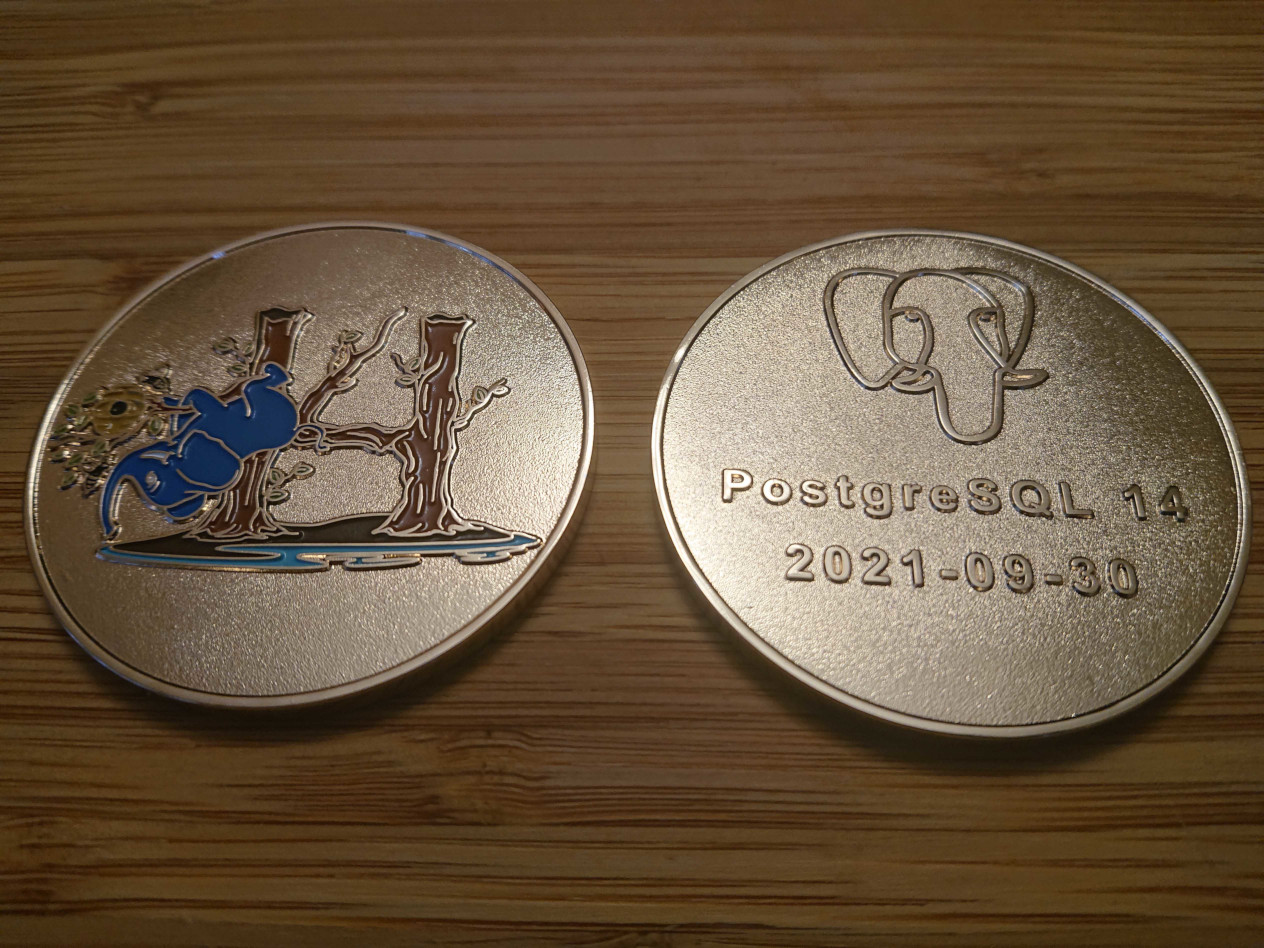
\includegraphics[width=\textwidth]{Pg14-challenge-coin.jpg}
      \end{center}
    \end{column}
  \end{columns}

  \vspace{.3cm}

  \footnotesize
  
\includegraphics[height=1cm]{qr-pg14-ack.png}
  \url{https://www.postgresql.org/docs/14/release-14.html#RELEASE-14-ACKNOWLEDGEMENTS}
}

\frame[containsverbatim]
{
  \frametitle{Anticipation of Initial Questions}

  \begin{columns}
    \begin{column}[T]{.333\textwidth}
      \begin{center}
        Am I in the release notes?
      \end{center}
    \end{column}
    \begin{column}[T]{.333\textwidth}
      \begin{center}
        What is the gift?
      \end{center}
    \end{column}
    \begin{column}[T]{.333\textwidth}
      \begin{center}
        How do I get it?
      \end{center}
    \end{column}
  \end{columns}

  \vspace{1cm}

  See \textbf{Contributors Gifts} on the community wiki for links to each
  releases' Acknowledgements, photos of the gifts, and how to claim your gift:
  \url{https://wiki.postgresql.org/wiki/Contributor_Gifts} 

  \begin{center}
    
\includegraphics[height=1cm]{qr-contributor-gifts.png}
  \end{center}
}

\frame
{
  \frametitle{Story Time}

  \Large
  \begin{center}
    Part 1: Writing the Acknowledgements
  \end{center}

  \begin{center}
    Part 2: Creating and distributing the gifts
  \end{center}
}

\frame
{
  \Huge
  \begin{center}
    Part 1:

    Writing the Acknowledgements
  \end{center}
}

\frame
{
  \frametitle{How contributions are recognized for the Release Notes}

  Peter Eisentraut, Corey Huinker et al. review thousands of commits to
  identify:

  \begin{columns}
    \begin{column}[T]{.5\textwidth}
      \begin{itemize}
        \item Patch authors - Includes documentation as well as code patches
        \item Reviewers
        \item Testers
        \item Bug reporters
      \end{itemize}
    \end{column}
    \begin{column}[T]{.5\textwidth}
      Number acknowledged:
      \begin{itemize}
        \item v12 - 410
        \item v13 - 380
        \item v14 - 411
        \item v15 - 411
        \item v16 - 382
        \item v17 - 476
        \item v18 - 527
      \end{itemize}
    \end{column}
  \end{columns}
}

\frame
{
  \Huge
  \begin{center}
    Part 2:

    Creating

    and

    distributing the gifts
  \end{center}
}

\frame[containsverbatim]
{
  \frametitle{Artwork}

  Artwork for each major release has been commissioned over the years and is
  used for the contributor gifts, in addition to other swag:

   
\includegraphics[height=1cm]{qr-artwork.png}
   \url{https://wiki.postgresql.org/wiki/Artwork}

  \begin{center}
    
\includegraphics[height=3.5cm]{postgresql-18.png}
    
\includegraphics[height=3.5cm]{postgresql-17.png}
    
\includegraphics[height=3.5cm]{postgresql-16.png}
    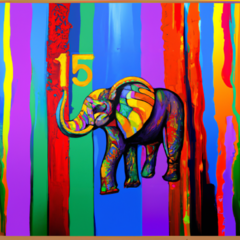
\includegraphics[height=3.5cm]{postgresql-15.png}
  \end{center}
}

\frame[containsverbatim]
{
  \frametitle{Commissioning Artwork}

  \begin{columns}
    \begin{column}[T]{.5\textwidth}
      \begin{itemize}
        \item Design Contests (generally frowned upon)
        \item Engaging artists or agencies directly
        \item Themes
        \begin{itemize}
          \item Elephant
          \item Release number
          \item May include a pun, homonyms, or play on words
        \end{itemize}
      \end{itemize}
    \end{column}
    \begin{column}[T]{.5\textwidth}
      \begin{itemize}
        \item Transfer of ownership to PostgreSQL Community Association (PGCA)
        \item PGCA is a Canada non-profit organization for protecting the
              PostgreSQL project's trademarks and brand assets
        \item https://www.postgres.ca/
              
\includegraphics[height=1cm]{qr-pgca.png}
      \end{itemize}
    \end{column}
  \end{columns}
}

\frame[containsverbatim]
{
  \frametitle{Challenge Coin}

  A \textbf{challenge coin}, also known as \textbf{memorial coin}, is a small
  coin or medallion, bearing an organization's insignia or emblem and carried
  by the organization's members.

  %\url{https://en.wikipedia.org/wiki/Challenge_coin}

  \begin{center}
  %  
\includegraphics[height=1cm]{qr-challenge-coin.png}
    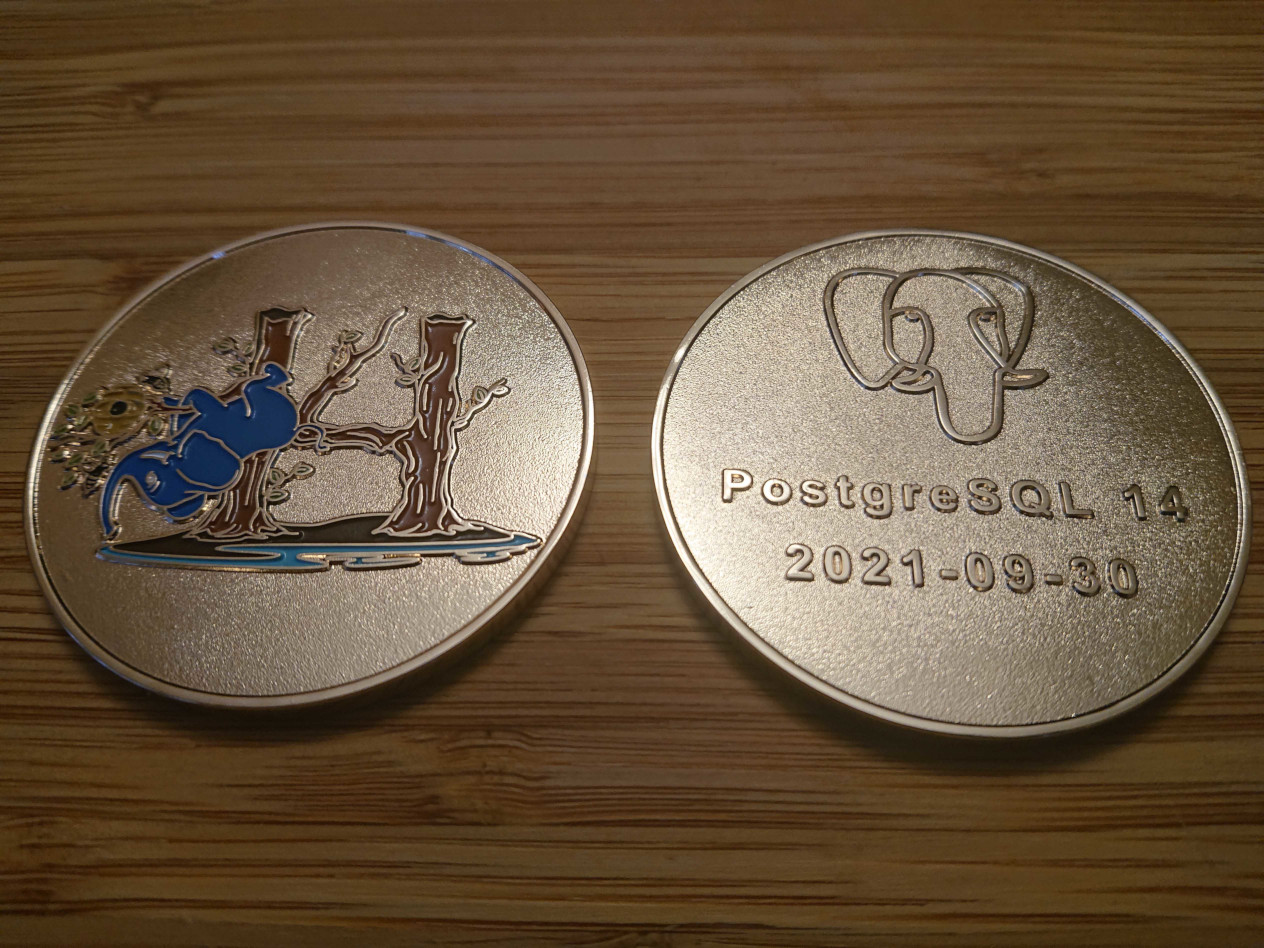
\includegraphics[scale=.6]{Pg14-challenge-coin.jpg}
  \end{center}
}

\frame
{
  \frametitle{Distribution}

  Gifts must be claimed each year:
  \begin{itemize}
    \item Email address obtained from public mailing lists
    \item Contributors contacted for their mailing address
    \item Word of mouth
    \item Handed out at some PostgreSQL events
    \item Volunteers help mail all around the world
  \end{itemize}
}

\frame[containsverbatim]
{
  \frametitle{How is it funded?}

  \begin{itemize}
    \item PostgreSQL\textsuperscript{\textregistered} Funds Groups\\
          
\includegraphics[height=1cm]{qr-funds-group.png}
          \url{https://www.postgresql.org/about/policies/funds-group/}
    \item A proposal is made
    \begin{itemize}
      \item Estimate of costs
      \begin{itemize}
        \item The gift itself
        \item Postage
        \item Shipping supplies
      \end{itemize}
    \end{itemize}
    \item The Funds Groups votes
    \item If the motion passes, then the gifts are purchased
  \end{itemize}
}

\frame[containsverbatim]
{
  \begin{center}
    \Huge
    Thank you!\\
    \rule{0.25\textwidth}{0.5pt}
  \end{center}

  \begin{center}
    Mark Wong\\
    PostgreSQL Major Contributor\\
    markwkm@postgresql.org\\
    \vspace{.2cm}
    
\includegraphics[height=1cm]{qr-markwkm.png}\\
    \rule{0.25\textwidth}{0.5pt}
  \end{center}

  \note[item]{This is a note.}
}

\end{document}
